\begin{frame}
\frametitle{Userspace vs kernelspace}
\begin{itemize}
  \item<1-> kernelspace (о нем вы уже знаете):
    \begin{itemize}
      \item kernelspace код использует наивысший приоритет исполнения (на x86 $CPL==0$);
      \item kernelspace память общая для всех процессов
        \begin{itemize}
          \item часть таблиц страниц процессов ссылаются на одну и ту-же память;
        \end{itemize}
      \item имеет неограниченный доступ ко всем ресурсам;
    \end{itemize}
  \item<2-> userspace (о нем вы еще не знаете):
    \begin{itemize}
      \item userspace код использует низший приоритет исполнения (на x86 $CPL==3$);
      \item userspace память своя у каждого процесса (с оговорками);
      \item для доступа к ресурсам должен спросить kernelspace;
      \item обычно приложения работают в userspace, чтобы они не мешали друг другу;
    \end{itemize}
\end{itemize}
\end{frame}

\begin{frame}
\frametitle{Приоритет исполнения}
\begin{itemize}
  \item<1-> Userspace код одного процесса не должен вредить другим процессам, например:
    \begin{itemize}
      \item userspace код не может менять таблицу страниц;
      \item userspace код не может менять GDT (специфично для x86);
    \end{itemize}
  \item<2-> Userspace не может выполнять некоторые инструкции:
    \begin{itemize}
      \item такие инструкции называют привилегированными;
      \item это инструкции изменяющие состояние системы;
      \item например, \emph{lgdt} или \emph{mov} в регистр \emph{cr3};
    \end{itemize}
\end{itemize}
\end{frame}

\begin{frame}
\frametitle{Userspace vs kernelspace memory}
\begin{figure}
  \centering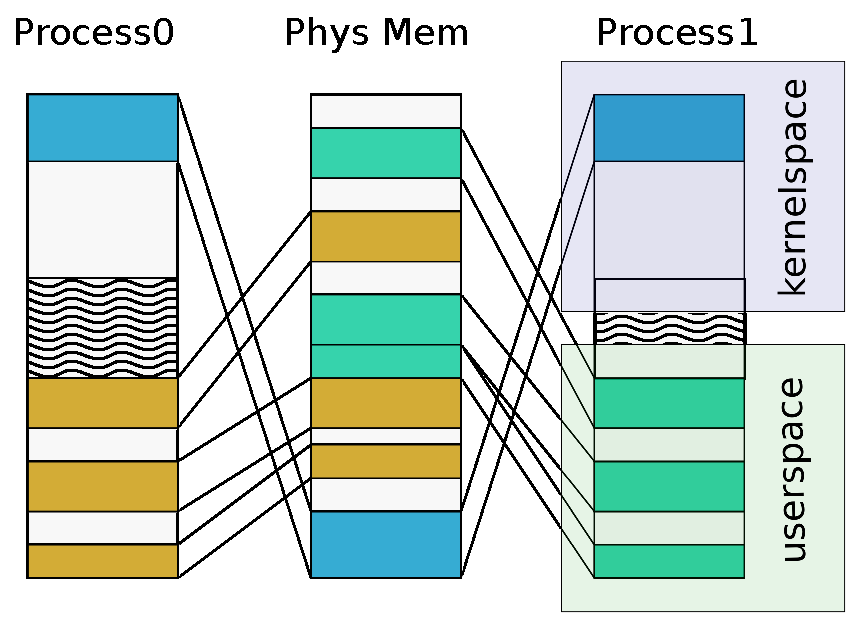
\includegraphics[width=.8\linewidth]{memory}
  \caption{Kernelspace vs Userspace Memory}
\end{figure}
\end{frame}

\begin{frame}
\frametitle{Передача управления между userspace и kernelspace}
\begin{itemize}
  \item<1-> Userspace сильно ограничен в возможностях, но он должен обращаться к ядру ОС
    \begin{itemize}
      \item нужна возможность передать управление в kernelspace;
      \item нельзя просто разрешить перейти в kernelspace;
      \item передать управление в kernelspace можно только определенному доверенному коду;
      \item доверенный код обрабатывает запрос от userspace кода;
    \end{itemize}
  \item<2-> Есть и обратная задача - передать управление из kernelspace в userspace:
    \begin{itemize}
      \item ядро ОС запускается в привилегированном режиме работы процессора;
      \item после обработки запроса в kernelspace, мы должны как-то вернуть управление в userspace;
    \end{itemize}
\end{itemize}
\end{frame}

\begin{frame}
\frametitle{Системные вызовы}
\begin{itemize}
  \item Системный вызов - интерфейс передающий управление между userspace и kernelspace кодом:
    \begin{itemize}
      \item userspace код сохраняет данные запроса в определенных (создателями ОС) местах, например, в регистрах;
      \item userspace код делает системный вызов (мы поговорим об это дальше);
      \item системный вызов производит переключение режима работы процессора и вызывает код ядра ОС (нужна аппаратная поддержка);
      \item код ядра ОС сохраняет все что нужно сохранить (например, volatile регистры) и обрабатывает запрос;
    \end{itemize}
\end{itemize}
\end{frame}

\begin{frame}
\frametitle{Реализация системных вызовов в x86}
\begin{itemize}
  \item Помните о прерываниях?
    \begin{itemize}
      \item при возникновении прерывания, управление передается обработчику прерывания ядра;
      \item прерывания можно генерировать специальной командой \emph{int};
      \item выделим неиспользуемый номер прерывания под системные вызовы;
      \item возврат из системного вызова - \emph{iret};
    \end{itemize}
\end{itemize}
\end{frame}

\begin{frame}
\frametitle{Смена привилегий в x86}
\begin{itemize}
  \item Если прерывание сгенерировано инструкцией \emph{int}, то процессор проверят поле \emph{DPL} дескриптора прерываний;
  \item \emph{CPL} (тот что в регистре \emph{CS}) должен быть меньше или равен \emph{DPL} в дескрипторе;
  \item таким образом userspace код может вызвать только системный вызов;
  \item для прерываний сгенерированных устройствами и исключений эта проверка не выполняется;
\end{itemize}
\end{frame}

\begin{frame}
\frametitle{Переключение стека в x86}
\begin{itemize}
  \item<1-> Обычно мы хотим, чтобы обработчик прерывания пользовался своим стеком, а не userspace стеком
    \begin{itemize}
      \item мы не хотим, чтобы userspace код мог потом прочитать со стека какие-то данные ядра ОС;
      \item мы не знаем, сколько стека использовал userspace и сколько осталось нам;
    \end{itemize}
  \item<2-> Поэтому, если обработчик прерывания прерывает userspace код нужно сменить стек:
    \begin{itemize}
      \item для этого (и многого другого) в x86 используется \emph{TSS};
    \end{itemize}
\end{itemize}
\end{frame}

\begin{frame}
\frametitle{Task State Segment}
\begin{itemize}
  \item В структуре \emph{TSS} хранится указатель стека, который будет загружен в \emph{RSP};
  \item обычно, в \emph{TSS} записывают вершину стека ядра потока исполнения и обновляют значение при переключении потоков;
  \item в \emph{GDT} должна быть специальная запись описывающая \emph{TSS};
  \item в специальный регистр \emph{TR} должен быть записан селектор \emph{TSS} дескриптора в \emph{GDT};
  \item формат \emph{TSS} описан в \emph{7.7 TASK MANAGEMENT IN 64-BIT MODE} документации \emph{Intel}
\end{itemize}
\end{frame}
